\begin{figure}[!tb]
\begin{center}
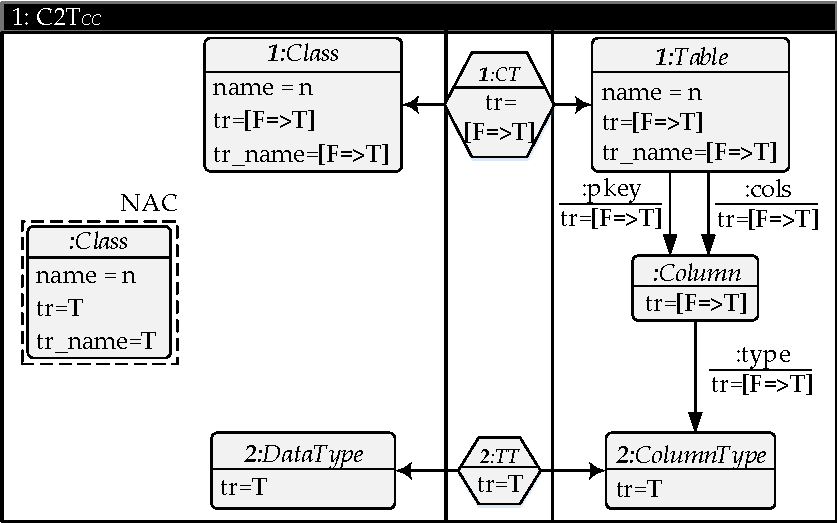
\includegraphics[width=.75\textwidth]{img/gen_intro/cc.pdf}
\end{center}
\caption{Consistency Creating Rule}
\label{fig:sec-msynch-tgg:cc_rule}
\end{figure}

Given a triple type graph $\TG=(\TG^\SRC \gets \TG^\C \to \TG^\T)$ with source domain $\Lang(\TG^\SRC)$ and target domain $\Lang(\TG^T)$ (cf. \cref{sec-dc-general,def:sec-dc-general:lang} for $\Lang(\TG^\SRC)$ and $\Lang(\TG^\T)$).
A source (target) model update\index{model update} $\delta$ on source graph $G \in \Lang(\TG^\SRC)$ (target graph $G \in \Lang(\TG^\T)$) is a span of inclusions $\delta=(G \transB{u_1} H \trans{u_2} G'),u_1,u_2 \in \M$ with $G,H,G' \in \Lang(\TG^\SRC)$ ($G,H,G' \in \Lang(\TG^\T)$).
Elements $G \setminus u_1(H)$ are deleted in $G$ whereas elements $G' \setminus u_2(H)$ are added to $G$.
With $\Delta^\SRC$ ($\Delta^\T$) we denote the set of all source (target) model updates.
A model synchronisation is a propagation of model updates from the source to the target domain via forward propagation operation $\fPpg$.
\index{model synchronisation}Operation $\fPpg$ takes a triple graph $(G^\SRC \gets G^\C \to G^\T)$ typed over $\TG$ together with a source model update $\delta^\SRC=(G^\SRC \gets H^\SRC \to G'^\SRC) \in \Delta^\SRC$ on $G^\SRC$ as input and outputs a target model update $\delta^\T=(G^\T \gets H^\T \to G'^\T) \in \Delta^\T$ on $G^\T$ together with a triple graph $(G'^\SRC \gets G'^\C \to G'^\T)$ typed over $\TG$ that interrelates the results $G'^\SRC$ and $G'^\T$ of both updates via correspondence $G'^\C$.
This corresponds to the informal description of model synchronisations in \cref{sec-gen-intro-msynch}.
The backward case of propagating updates from the target to the source domain via backward propagation operation $\bPpg$ is defined analogously and omitted in the following.
According to Def. 9.18 in \cite{FAGT2}, the synchronisation operation $\fPpg$ is a composition of three auxiliary operations $\fAln,\del$ and $\fAdd$.
For technical details we refer to Chapter 9 in \cite{FAGT2}.
Operation $\del$ relies on operational consistency creating (CC) rules \cite{DBLP:journals/sosym/0001EOCDXGE15}.
Similarly to forward translation rules in \cref{sec-mt-tgg,def:sec-mt-tgg:fwd_bwd_tr_rules}, the CC rule $\tr_\CC$ of a given triple rule $\tr$ does not create elements in the sense that it already contains all elements of $\tr$ including the created elements in the left-hand side and furthermore, each element that is created by $\tr$ is initially marked with translation attribute $\False$ und updated to $\True$, written $[\False => \True]$, while all other elements are initially marked with $\True$ and remain unchanged.
Rule \code{C2T}$_\CC$ in \cref{fig:sec-msynch-tgg:cc_rule} is the CC rule of triple rule \code{C2T} in \cref{sec-gt-trafo,fig:sec-gt-trafo:tgg}.
For CC rules we review the existing result in \cref{fact:sec-msynch-tgg:equ_tr_cc} which is used to prove \cref{sec-dc-verification,lem:equivalence-marking-emptySG}.

\begin{definition}[Consistency Creating (CC) Rule (Def. 7.44 in \cite{FAGT2})]
\label{def:sec-msynch-tgg:cc_rule}
\index{triple rule!consistency creating rule}
Given a triple rule $\tr=(L \to R,\ac_L)$, then \emph{the consistency creating rule $\tr_\CC$ of $\tr$} is given by $\tr_\CC=(L_\CC \transB{l_\CC} K_\CC \trans{r_\CC} R_\CC,\ac_\CC)$ with:
\begin{enumerate*}
  \item $L_\CC=(R \oplus \Att^\True_L \oplus \Att^\False_{R \setminus L})$,
  \item $K_\CC=(R \oplus \Att^\True_L)$,
  \item $R_\CC=(R \oplus \Att^\True_L \oplus \Att^\True_{R \setminus L})$,
  \item $l_\CC$ and $r_\CC$ are the induced inclusions, and
  \item $\ac_\CC=\tExt(\ac_L,L_\CC,\{S,C,T\})$.
\end{enumerate*}
With $\TR_\CC$ we denote the set of consistency creating rules $\tr_\CC$ of all triple rules $\tr \in \TR$ for a given set of triple rules $\TR$.
\envEndMarker
\end{definition}

\begin{figure}[!tb]
\begin{center}
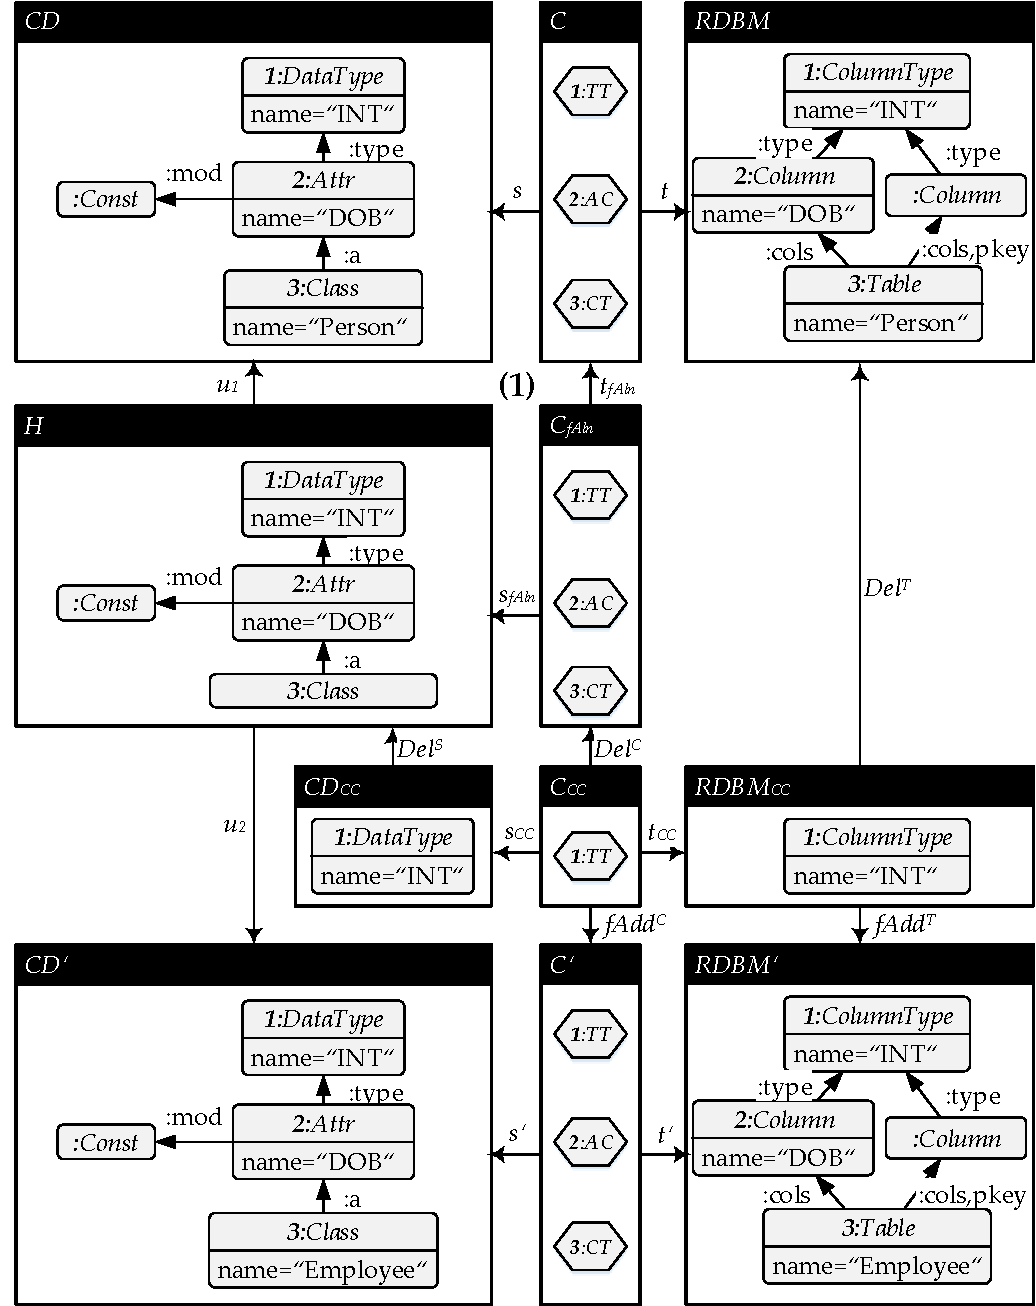
\includegraphics[width=.85\textwidth]{img/gen_intro/sync.pdf}
\end{center}
\caption{Model Synchronisation via Forward Propagation Operation $\fPpg$}
\label{fig:sec-msynch-tgg:fwd}
\end{figure}

\begin{remark}[Meta-Modelling \& Model Synchronisation]
Given the triple type graph $\TG=(\TG_\CD \gets \TG_C \to \TG_\RDBM)$ from \cref{fig:sec-gt-graphs:atg} with triple graph $G=(\CD \gets C \to \RDBM) \in \Lang(\TG)$ and source model update $\delta=(\CD \transB{u_1} H \trans{u_2} \CD')$ in \cref{fig:sec-msynch-tgg:fwd}, then $\fPpg(G,\delta)=(G',\delta')$ with $G'=(\CD' \transB{s'} C' \trans{t'} \RDBM') \in \Lang(\TG)$ and target model update $\delta'=(\RDBM \transB{\del^\T} \RDBM_\CC \trans{\fAdd^\T} \RDBM')$.
Target update $\delta'$ on $\RDBM$ reflects the change of source update $\delta$ on $\CD$ (the \code{name} of the \code{Class} is changed from \code{Person} to \code{Employee}) in the target domain.
The output $(G',\delta')$ is obtained by three sequential operations $\fAln,\del$ and $\fAdd$:
Alignment operation $\fAln$ creates pullback $(1)$ in order to align deletions of update $\delta$ to the correspondence component and yields triple graph $G_1=(H \transB{s_\fAln} C_\fAln \trans{t \circ t_\fAln} \RDBM)$.
Operation $\del$ creates the maximal consistently integrated triple sub-graph of $G_1$ by creating the graph $\Att^\False(G_1)$ with translation attributes over $G_1$ and applying CC rules $\TR_\CC$ as long as possible afterwards.
The maximal consistently integrated sub-graph is given by all $\True$-marked elements, i.e., by triple graph $G_2=(\CD_\CC \transB{s_\CC} C_\CC \trans{t_\CC} \RDBM_\CC)$ with inclusion $(\del^\SRC,\del^\C,\del^\T)\colon G_2 \to G_1$ (the translation attributes are omitted in \cref{fig:sec-msynch-tgg:fwd}).
Operation $\fAdd$ adds those elements to $G_2$ that are created by update $\delta$ leading to triple graph $G_3=(\CD' \transB{u_2 \circ \del^\SRC \circ s_\CC} C_\CC \trans{t_\CC} \RDBM_\CC)$ where additionally all elements that are creatd by $\delta$ are marked with translation attributes $\False$.
Finally, a complete forward translation sequence $G_3 \Trans{\tr^*_\FT} G'$ leads to output $(G',\delta')$.
\envEndMarker
\end{remark}

\begin{fact}[Equivalence of Triple and Extended Consistency Creating Sequences (Fact 10 in \cite{heocdx11})]
\label{fact:sec-msynch-tgg:equ_tr_cc}
Let $\TGG=(\varnothing,\TR)$ be a triple graph grammar typed over triple type graph $\ATGI$ with empty start graph $\varnothing$ and derived consistency creating rules $\TR_\CC$ of triple rules $\TR$.
Let $G \in \Lang(\ATGI)$ be a graph according to \cref{sec-dc-general,def:sec-dc-general:lang}, then the following are equivalent for almost injective matches $m \in \morO$.
\begin{itemize}
	\item There exists a consistency creating sequence $\Att^\False(G) \Trans{\tr_\CC^*} G \oplus \Att_{G_k}^\True \oplus \Att_{G \setminus G_k}^\False$ via consistency creating rules $\TR_\CC$.% with intermediate steps $(G'_i \Trans{(m_i,m(p_i))} G'_{i+1})$, where $m(p_i)=(L_i \xhookleftarrow{} K_i \xhookrightarrow{} R_i)$ and $\quotient{m_i}{L_i^{\False}}$ is type strict
	\item There exists a triple graph transformation $\varnothing \Trans{\tr^*} G_k$ via $\TR$ with injective embedding $f\colon G_k \to G$.% with intermediate steps $G_i \Trans{(m_i,p_i)} G_{i+1}$.
\envEndMarker
\end{itemize}
\end{fact}

\paragraph*{General Assumption}
Note that the definition of CC rules is based on attributions in attributed graphs.
Therefore, we assume all general assumptions from \cref{rem:sec-mt-tgg:gen_ass}. 